\documentclass{amsart}

\usepackage{fullpage, amsmath, amssymb, amsthm, enumitem, tabularx, multirow, multicol, tikz, venndiagram, graphicx}
\renewcommand{\baselinestretch}{1.15}

\title{Math Concepts_2_Functions}
\author{Emre Usenmez}
\thanks{Gonville \verb|&| Caius College. Extremely grateful to Prof Jay Cummings as these notes made liberal use of his book 'Proofs'.}
\date{August 2023}

\newtheorem{thrm}{Theorem}
\theoremstyle{definition}
\newtheorem*{dfn}{Definition}
\theoremstyle{definition}
\newtheorem*{prpn}{Proposition}
\theoremstyle{remark}
\newtheorem*{note}{Note}

\usepackage{Sweave}
\begin{document}
\Sconcordance{concordance:Math_Concepts_2_Functions.tex:Math_Concepts_2_Functions.Rnw:1 %
18 1 1 0 71 1}


\begin{center}
      \textbf{TOPIC TWO: FUNCTIONS}
\end{center}

In Topic One we studied the static properties of sets. Things get more dynamic when we start applying functions to those sets.

\section{\textbf{Definitions}}
\begin{dfn}
      \boxed{f:A \rightarrow B} \quad Given a pair of sets $A$ and $B$, suppose that each element $x \in A$ is associated, in some way, to a unique element of $B$, which we denote $f(x)$. Then $f$ is said to be a \emph{function} from $A$ to $B$. This is often denoted
      \[ f: A \rightarrow B \]
      which is typically read "$f$ from $A$ to $B$."
      \begin{flalign*} % used flalign instead of align to left-justify the text and not center it. Lines within each flalign should begin and end with &.
            \text{Furthermore, }
            &A \text{ is called the \emph{domain} of } f, && \text{(can be though of as inputs of $f$)} & \\
            &B \text{ is called the \emph{codomain} of } f, \text{ and} && \text{(\dots as a set to which all outputs belong)} & \\
            &\text{The set } \{f(x):x \in A\} \text{ is called the \emph{range} of } f. && \text{(\dots as outputs of $f$)}
      \end{flalign*}
      All three correspond to each other via $f$ but they are just sets. \\
      Range consists only of elements in the codomain that gets mapped. That is, $y$ is in the range if there is an $x$ in the domain that maps to it: $f(x) = y$. For e.g.,
      \begin{itemize}
            \item if $f : \mathbb{R} \rightarrow \mathbb{R}$ is given by $f(x) = 2x$ then the range is $\mathbb{R}$.
            \item if $f : \mathbb{R} \rightarrow \mathbb{R}$ is given by $f(x) = x^2$ then the range is the set of nonnegative real numbers: ie, the interval $[0, \infty)$.
      \end{itemize}
\end{dfn}

A function's domain and codomain can each be any set. Here is a graphical way to write som function $f$:

\begin{figure}[h] %The optional argument to the figure environment tells LaTeX where you'd like it to appear, if possible; the options are h meaning "here", t (at the top of a page), b (at the bottom of a page) and p (on a page without any text). This is only a suggestion to LaTeX, and it might ignore it if it doesn't think your instruction can be done neatly. If you want to encourage LaTeX to take your suggestion seriously you can put an exclamation mark before the location, e.g. \begin{figure}[!b].
      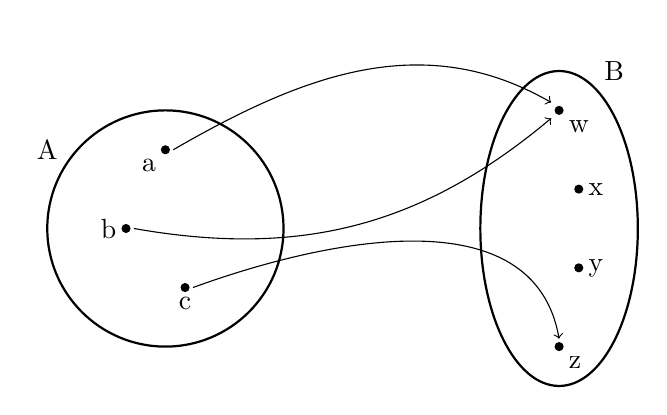
\begin{tikzpicture}
            \draw [thick] (1,0) circle (1.5cm); %This large circle contains points a, b, c
                  \node at (-0.5,1) {A}; % This produces the set name A
            \draw[thick] (6,0) ellipse (1cm and 2cm);
                  \node at (6.7,2) {B};

            \draw[fill] (1,1) circle [radius = 0.05]; %This is the dot we will label a
                  \node [below left] at (1,1) {a}; % We name the dot a and locate it below left of (1,1)
            \draw [fill] (0.5, 0) circle [radius = 0.05];
                  \node [left] at (0.5, 0) {b};
            \draw[fill] (1.25,-0.75) circle [radius = 0.05];
                  \node[below] at (1.25,-0.75) {c};

            \draw[fill] (6, 1.5) circle [radius = 0.05];
                  \node[below right] at (6, 1.5){w};
            \draw[fill](6.25, 0.5) circle [radius = 0.05];
                  \node[right] at (6.25, 0.5){x};
            \draw[fill](6.25, -0.5) circle [radius = 0.05];
                  \node[right] at (6.25, -0.5){y};
            \draw[fill](6, -1.5) circle [radius = 0.05];
                  \node[below right] at (6, -1.5){z};

            \draw[->] (1.1,1) to [out=30, in=150] (5.9, 1.6); % arrow from a to w with curve degrees.
            \draw[->] (0.6, 0) to [out=-10, in=220] (5.9, 1.4); % arrow from b to w with curve degrees.
            \draw[->] (1.35, -0.75) to [in=100, out=20] (6, -1.4); %arrow from c to z with curve degrees.
      \end{tikzpicture}
    \caption{A function $f: A \rightarrow B$}
            \label{fig:function_diagram} %allows us the refer to this figure later on even if the figure numbering changes it keeps references correct.
\end{figure}

Figure \ref{fig:function_diagram} above illustrates a function with \emph{domain} \{a, b, c\}, \emph{codomain} \{w, x, y, z\}, and \emph{range} \{w, z\}.
\begin{note}
      There does not exist any $k \in \{a, b, c\}$ such that $f(k)=y$, which is why $y$ is not in the range.
\end{note}

For diagrams such as Figure \ref{fig:function_diagram} to represent a function, it would have to satisfy both existence and uniqueness aspects of a function. If it fails to do so, then it would not represent a function. For e.g., if $b$ did not map onto any of the elements in $B$ in Figure \ref{fig:function_diagram} then the diagram would not satisfy the existence condition - since $b$ is being sent to nowhere - and thus not represent a function. Similarly, if $b$ not only mapped onto $w$ but also onto $y$ simultaneously then it would not satisfy the uniqueness condition and the diagram would again not represent a function.

\begin{dfn}
\boxed{injection} \quad A function $f : A \rightarrow B$ is \emph{injective}, or one-to-one, if $f(a_1)=f(a_2)$ implies that $a_1=a_2$. For e.g.,
\begin{center}
\begin{tabular}{c c c}
      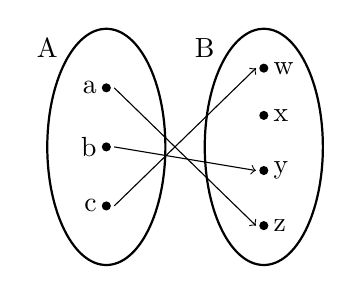
\begin{tikzpicture}
            \draw[thick] (1,1) ellipse (0.75cm and 1.5cm);
                \node at (0.25, 2.25){A};
            \draw[thick] (3,1) ellipse (0.75cm and 1.5cm);
                \node at (2.25, 2.25){B};

            \draw[fill] (1, 1.75) circle [radius=0.05];
                \node[left] at (1, 1.75){a};
            \draw[fill] (1, 1) circle [radius=0.05];
                \node[left] at (1, 1){b};
            \draw[fill] (1, 0.25) circle [radius=0.05];
                \node[left] at (1, 0.25){c};

            \draw[fill] (3, 2) circle [radius=0.05];
                \node[right] at (3, 2){w};
            \draw[fill] (3, 1.4) circle [radius=0.05];
                \node[right] at (3, 1.4){x};
            \draw[fill] (3, 0.7) circle [radius=0.05];
                \node[right] at (3, 0.7){y};
            \draw[fill] (3, 0) circle [radius=0.05];
                \node[right] at (3, 0){z};

            \draw[->] (1.1,1.75) to (2.9,0);
            \draw[->] (1.1,1) to (2.9,0.7);
            \draw[->] (1.1,0.25) to (2.9,2);

      \end{tikzpicture}
      &
      &
      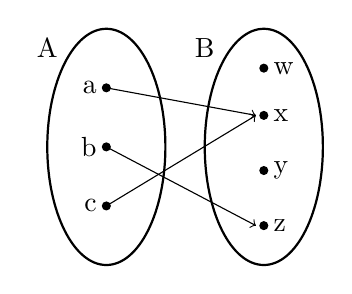
\begin{tikzpicture}
            \draw[thick] (6,1) ellipse (0.75cm and 1.5cm);
                \node at (5.25, 2.25) {A};
            \draw[thick] (8,1) ellipse (0.75cm and 1.5cm);
                \node at (7.25, 2.25){B};

            \draw[fill] (6, 1.75) circle [radius=0.05];
                \node[left] at (6, 1.75){a};
            \draw[fill] (6, 1) circle [radius=0.05];
                \node[left] at (6, 1){b};
            \draw[fill] (6, 0.25) circle [radius=0.05];
                \node[left] at (6, 0.25){c};

            \draw[fill] (8, 2) circle [radius=0.05];
                \node[right] at (8, 2){w};
            \draw[fill] (8, 1.4) circle [radius=0.05];
                \node[right] at (8, 1.4){x};
            \draw[fill] (8, 0.7) circle [radius=0.05];
                \node[right] at (8, 0.7){y};
            \draw[fill] (8, 0) circle [radius=0.05];
                \node[right] at (8, 0){z};

            \draw[->] (6,1.75) to (7.9, 1.4);
            \draw[->] (6,1) to (7.9,0);
            \draw[->] (6, 0.25) to (7.9, 1.4);
      \end{tikzpicture} \\
    An injection from $A$ to $B$ &
    &
    Not an injection from $A$ to $B$
\end{tabular}
\end{center}

\bigskip
Both of these are functions. However, the second one is not injective because $f(a)=x$ and $f(c)=x$, which means $f(a) = f(c)$ while $a \neq c$, as these are distinct elements in the domain. Basically, to be injective means that you do not have two arrows pointing at the same point. \\
This can also be shown via contrapositive:
\[ \text{A function } f:A\rightarrow B \text{ is \emph{injective}, or one-to-one, if } a_1 \neq a_2 \text{ implies that } f(a_1) \neq  f(a_2). \]

So a function is \emph{injective} if different points in the domain are sent to different points in the codomain. No two arrowheads collide.
\end{dfn}

\begin{dfn}
\boxed{surjection} \quad A function $f:A \rightarrow B$ is \emph{surjective}, or onto, if, for every $b \in B$, there exists some $a \in A$ such that $f(a)=b$. For e.g.,

\medskip

\begin{center}
\begin{tabular}{c c c}
      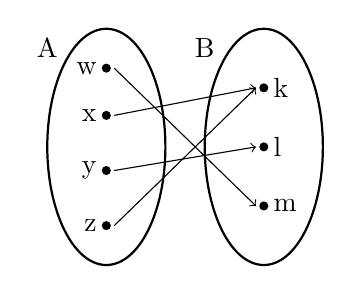
\begin{tikzpicture}
            \draw[thick] (1,1) ellipse (0.75cm and 1.5cm);
                \node at (0.25, 2.25){A};
            \draw[thick] (3,1) ellipse (0.75cm and 1.5cm);
                \node at (2.25, 2.25){B};

            \draw[fill] (1, 2) circle [radius=0.05];
                \node[left] at (1, 2){w};
            \draw[fill] (1, 1.4) circle [radius=0.05];
                \node[left] at (1, 1.4){x};
            \draw[fill] (1, 0.7) circle [radius=0.05];
                \node[left] at (1, 0.7){y};
            \draw[fill] (1, 0) circle [radius=0.05];
                \node[left] at (1, 0){z};

            \draw[fill] (3, 1.75) circle [radius=0.05];
                \node[right] at (3, 1.75){k};
            \draw[fill] (3, 1) circle [radius=0.05];
                \node[right] at (3, 1){l};
            \draw[fill] (3, 0.25) circle [radius=0.05];
                \node[right] at (3, 0.25){m};

            \draw[->] (1.1,2) to (2.9,0.25);
            \draw[->] (1.1,1.4) to (2.9,1.75);
            \draw[->] (1.1,0.7) to (2.9,1);
            \draw[->] (1.1,0) to (2.9,1.75);

      \end{tikzpicture}
      &
      &
      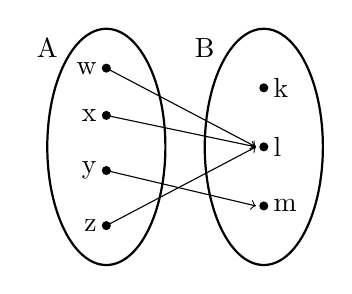
\begin{tikzpicture}
            \draw[thick] (6,1) ellipse (0.75cm and 1.5cm);
                \node at (5.25, 2.25) {A};
            \draw[thick] (8,1) ellipse (0.75cm and 1.5cm);
                \node at (7.25, 2.25){B};

            \draw[fill] (6, 2) circle [radius=0.05];
                \node[left] at (6, 2){w};
            \draw[fill] (6, 1.4) circle [radius=0.05];
                \node[left] at (6, 1.4){x};
            \draw[fill] (6, 0.7) circle [radius=0.05];
                \node[left] at (6, 0.7){y};
            \draw[fill] (6, 0) circle [radius=0.05];
                \node[left] at (6, 0){z};

            \draw[fill] (8, 1.75) circle [radius=0.05];
                \node[right] at (8, 1.75){k};
            \draw[fill] (8, 1) circle [radius=0.05];
                \node[right] at (8, 1){l};
            \draw[fill] (8, 0.25) circle [radius=0.05];
                \node[right] at (8, 0.25){m};

            \draw[->] (6,2) to (7.9, 1);
            \draw[->] (6,1.4) to (7.9,1);
            \draw[->] (6, 0.7) to (7.9, 0.25);
            \draw[->] (6, 0) to (7.9, 1);
      \end{tikzpicture} \\
    A surjection from $A$ to $B$ &
    &
    Not a surjection from $A$ to $B$
\end{tabular}
\end{center}

\bigskip
The diagram on the right does not satisfy the definition of \emph{surjection} because it is not true that for every $b \in \{k, l, m\}$ there ought to exist some $a \in \{w, x, y, z\}$ such that $f(a)=b$, but $b=k$ does not have this property. \\
In terms of arrows, this means every dot in $B$ has at least one arrow pointing at it. \\
As was the case for injection, surjection can also be defined using contrapositive:
\begin{center}
A function $f:A\rightarrow B$ is \emph{surjective}, or onto, if there does not exist any $b \in B$ for which $f(a)\neq b$ for all $a \in A$.
\end{center}
\end{dfn}

\begin{note}
When defining a function $f: A\rightarrow B$, the ideas of \emph{existence} and \emph{uniqueness} were focused on $A$ --- for every $x\in A$, we demand that $f(x)$ exists and be unique. To be injective and surjective, the attention shifts to $B$. To be \emph{surjective} means that $B$ has an existence criterion (for every $b\in B$, there \emph{exists} some $a\in A$ that maps to it). To be \emph{injective} means that $B$ has a uniqueness-type criterion (for every $b\in B$, there is \emph{at most one} $a\in A$ that maps to it).
\end{note}

\begin{dfn}
      \boxed{bijection} \quad A function $f:A\rightarrow B$ is \emph{bijective} if it is both injective and surjective.
      Being bijective means that every element in $A$ is paired up with precisely one element in $B$.

\bigskip
If we use the pairing analogy, simply by being a function everyone in $A$ has found someone to be in a relationship with. Surjectivity guarantees that everyone in $B$ has also found someone to pair up with. Injectivity means all the relationships are monogamous. Therefore being bijective means everyone is in a monogamous relationship.

In terms of arrows, being a bijection means that every dot on the left has precisely one arrow emanating from it, and every dot on the right has precisely one arrow entering it.

\end{dfn}

\begin{note}
      Defining a function $f:A\rightarrow B$ placed an existence and uniqueness criteria on $A$. If $f$ is both injective and surjective, then this adds existence and uniqueness criteria to $B$. Thus, if $f$ is a bijection, then it has these criteria on both sides: Every $a \in A$ is mapped to precisely one $b \in B$, and every $b\in B$ is mapped to precisely one $a \in A$. In effect, this pairs up each element of $A$ with an element of $B$; namely, $a$ is paired with $f(a)$ in this way.
\end{note}













\bigskip \bigskip

\subsection{\underline{Proving $x$jectiveness, for $x\in$\{in, sur, bi\}}}\hspace*{\fill}

In order to prove injectiveness and surjectiveness we will use their definitions. The outline to prove a function is injective is as follows.

\begin{prpn}
      $f:A\rightarrow B$ is an injection.
\end{prpn}

\begin{proof}
      Assume $x,y\in A$ and $f(x)=f(y)$.

      \begin{center}
            \guillemotleft\ An explanation of what $x,y\in A$ and $f(x)=f(y)$ means \guillemotright
      \end{center}

            \begin{center}
            \begin{tabular}{r l}
                  \multirow{3}{*}{\huge $\updownarrow$} & apply algebra \\
                  & apply logic \\
                  & apply techniques \\
            \end{tabular}
            \end{center}

            \begin{center}
                  \guillemotleft\ Oh hey look, that's what $x=y$ means \guillemotright
            \end{center}

            Therefore $x = y$.

            Since $x,y\in A$ and $f(x)=f(y)$ implies that $x = y$, it follows that $f$ is injective.

\end{proof}

Alternatively, we could also use the contrapositive where we would start by assuming $x\neq y$, and then conclude that $f(x) \neq f(y)$.


The outline for proving surjectiveness similarly uses its definition:

\begin{prpn}
      $f:A\rightarrow B$ is a surjection.
\end{prpn}

\begin{proof}
      Assume $b \in B$.

            \begin{center}
            \begin{tabular}{r l}
                  \multirow{2}{*}{\huge $\updownarrow$} & Find an $a \in A$ where $f(a)=b$, \\
                  & and show how it works \\
            \end{tabular}
            \end{center}

            Since every $b\in B$ has an $a \in A$ where $f(a) = b$, it follows that $f$ is surjective.

\end{proof}

To prove a function is a bijection, we can prove both above. \\
Let's apply these to some examples.








\bigskip \bigskip

\subsubsection{\underline{Proving injectiveness, surjectiveness, or bijectiveness of $x^2$}}\hspace*{\fill}
\bigskip

Let $\mathbb{R^+}$ denote the nonnegative real numbers. Lets prove the following:
\begin{enumerate}[label=(\alph*)]
      \item $f : \mathbb{R} \rightarrow \mathbb{R}$ where $f(x)=x^2$ is not injective, surjective, or bijective.
      \item $g : \mathbb{R^+} \rightarrow \mathbb{R}$ where $g(x)=x^2$ is injective, but not surjective or bijective.
      \item $h : \mathbb{R} \rightarrow \mathbb{R^+}$ where $h(x)=x^2$ is surjective, but not injective, or bijective.
      \item $k : \mathbb{R^+} \rightarrow \mathbb{R^+}$ where $k(x)=x^2$ is injective, surjective, and bijective.
\end{enumerate}

Notice that even though each function squares its input $x$, they are all different. This is because a function is not only the operation, but the domain and codomain as well. Since their domains and/or codomains do not match, they are all different functions. This allows them to have different properties, as we are proving here.

\bigskip
\noindent \textbf{Scratch Work.} The injective property is essentially a "horizontal line test". If every horizontal line through the range hits the function in only one place, the function is injective. But if any horizontal line through the range hits the function in more than one place, then the function is not injective because it wouldn't satisfy the uniqueness criterion.

\begin{center}
\begin{tabular}{c c c}

      \begin{tikzpicture}
            \draw[<->] (-2.5,0) -- (2.5,0) node[right] {$\mathbb{R}$};
            \draw[<->] (0,-0.5) -- (0,2.5) node[above left] {$\mathbb{R}$};
            \draw[<->, scale=0.5, domain=-2:2, smooth, variable=\x,] plot ({\x}, {\x*\x}) node[left] {$f(x)$}; %scaled it by half to fit in page. plot command is in (x,y) format where y=x^2.
            \draw[ultra thin, <->] (-2,0.5) -- (2,0.5);
            \draw[fill] (-0.5,0.5) circle [radius=0.05];
            \draw[fill] (0.5,0.5) circle [radius=0.05];
      \end{tikzpicture}
      &
      &
      \begin{tikzpicture}
            \draw[->] (0,0) -- (2.5,0) node[right] {$\mathbb{R^+}$};
            \draw[<->] (0,-0.5) -- (0,2.5) node[above left] {$\mathbb{R}$};
            \draw[<->, scale=0.5, domain=0:2, smooth, variable=\x,] plot ({\x}, {\x*\x}) node[below right] {$g(x)$};
            \draw[ultra thin, ->] (0,0.5) -- (2,0.5);
            \draw[ultra thin, ->] (0,2) -- (2,2);
            \draw[fill] (0,0) circle [radius=0.05];
            \draw[fill] (0.5,0.5) circle [radius=0.05];
            \draw[fill] (1,2) circle [radius=0.05];
      \end{tikzpicture}
      \\
      \begin{tikzpicture}
            \draw[<->] (-2.5,0) -- (2.5,0) node[right] {$\mathbb{R}$};
            \draw[<->] (0,0) -- (0,2.5) node[above left] {$\mathbb{R^+}$};
            \draw[<->, scale=0.5, domain=-2:2, smooth, variable=\x,] plot ({\x}, {\x*\x}) node[left] {$h(x)$};
            \draw[ultra thin, <->] (-2,0.5) -- (2,0.5);
            \draw[fill] (-0.5,0.5) circle [radius=0.05];
            \draw[fill] (0.5,0.5) circle [radius=0.05];
      \end{tikzpicture}
      &
      &
      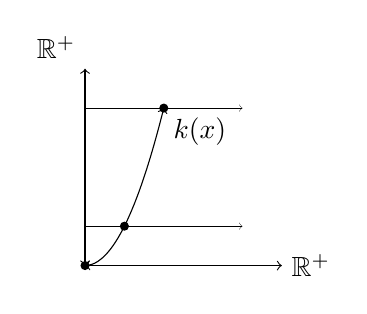
\begin{tikzpicture}
            \draw[->] (0,0) -- (2.5,0) node[right] {$\mathbb{R^+}$};
            \draw[<->] (0,0) -- (0,2.5) node[above left] {$\mathbb{R^+}$};
            \draw[<->, scale=0.5, domain=0:2, smooth, variable=\x,] plot ({\x}, {\x*\x}) node[below right] {$k(x)$};
            \draw[ultra thin, ->] (0,0.5) -- (2,0.5);
            \draw[ultra thin, ->] (0,2) -- (2,2);
            \draw[fill] (0,0) circle [radius=0.05];
            \draw[fill] (0.5,0.5) circle [radius=0.05];
            \draw[fill] (1,2) circle [radius=0.05];
      \end{tikzpicture}
\end{tabular}
\end{center}

Looking at the graphs, it makes sense that $f$ and $h$ are not injective since we can show that any two points from the domain do map to the same value in the codomain (for example, -1 and 1). On the other hand, $g$ and $k$ seems to be injective.


To prove that $g$ and $k$ are injective, we will assume that, say, $g(x)=g(y)$, and we will try to prove $x=y$:

\[ g(x) = g(y)\]
\[ x^2 = y^2 \]
\[ \sqrt{x^2} = \sqrt{y^2} \]
\[x = y \text{ or } x=-y\]

While $x$ take on two values, $y$ and $-y$, and thus violates the uniqueness criterion for $f$ and $h$, this is not the case for $g$ and $k$ since their domains do not include negative numbers. So, for $g$ and $k$ this scratch work should prove $x=y$, which would in turn prove these functions are injective.


For surjectivity, or at least to show that a function is not surjective, we need to find some $y$ in the codomain that nothing maps to. Since functions $f$ and $g$ has $y$s that are negative, and there aren't any $x$s square of which would be negative, we can easily show that $f$ and $g$ are not surjective. On the other hand, the codomains of $h$ and $k$ do not include negative numbers so they will be surjective. To show this, we will pick any $y$ in the codomain, and find the specific $x$ in the domain such that $h(x)=y$ and $k(x)=y$. The value of $x = \sqrt{y}$ should work in both cases.

\bigskip
\begin{proof}
      \underline{Part i.} \quad Observe that $f(-2) = f(2)$ while $-2 \neq 2$, showing that $f$ is not injective. \\
      Also observe that $f(x)=x^2 \geq 0$ for all $x \in \mathbb{R}$ showing that there does not exist $x \in \mathbb{R}$ for which $f(x) = -4$ --- or for which $f(x)  < 0$. Since -4, and all negative numbers, are in $f$'s codomain, this proves that $f$ is not surjective, either. \\
      Since $f$ is not surjective or injective, it cannot be bijective either.


      \medskip
      \underline{Part ii.} \quad Observe that $g(x)=x^2 \geq 0$ for all $\mathbb{R^+}$, there does not exist $x \in\mathbb{R}$ for which $g(x) = -4$ --- or for which $f(x)  < 0$. Since -4, and all negative numbers, are in $g$'s codomain, this proves that $g$ is not surjective. \\
      By definition, this also means $g$ is not bijective. \\
      To see $g$ is injective, assume $x,y\in \mathbb{R^+}$ and $g(x)=g(y)$. Then,
      \[ g(x) = g(y) \]
      \[ x^2 = y^2 \]
      \[ \sqrt{x^2} = \sqrt{y^2} \]
      \[x = y \text{ or } x=-y\]

      Since $x,y\in\mathbb{R^+}$, the only option is that both $x$ and $y$ can only be positive, so $x=y$. \\
      We have shown that $g(x)=g(y)$ implies $x=y$, thus $g$ is an injection.


      \medskip
      \underline{Part iii.} \quad Observe that $h(x)$ is not injective for the same reasons as $f$: $f(-2)=f(2)$ but $-2 \neq 2$ showing that $h$ is not injective. \\
      This means, by definition, it cannot be bijective, either. \\
      To show that $h$ is a surjection, pick any $y$ in its codomain, $\mathbb{R^+}$, and note that its positive square root exists since $y \geq 0$. If that positive square root is $x$, then $x\in\mathbb{R^+}$ since $x=\sqrt{y}$. Therefore,
      \[h(x) = x^2 = (\sqrt{y}^2) = y. \]
      We have shown that for every $b\in\mathbb{R^+}$ there exists an $x\in\mathbb{R^+}$ such that $h(x)=y$. This proves that $h$ is a surjection.


      \medskip
      \underline{Part iii.} \quad The fact that $k$ is an injection follows the same reasoning as with $g$ in Part ii, and the fact that $k$ is a surjection follows the exact same reasoning as with $h$ in Part iii. Since $k$ is an injection and a surjection, it is also a bijection.

\end{proof}

\bigskip
As it may be clear from the above proof that it is easier and shorter to prove that a function is not an injection or surjection. We need one counterexample to prove that a function violates their criteria.




\bigskip \bigskip

\subsubsection{\underline{Proving bijectiveness of $f(x,y)=(x+2y, 2x+3y)$}}\hspace*{\fill}
\medskip

\begin{prpn}
      The function $f:(\mathbb{Z}\times\mathbb{Z}) \rightarrow (\mathbb{Z}\times\mathbb{Z})$ where $f(x,y) = (x+2y, 2x+3y)$ is a bijection.
\end{prpn}

\noindent \textbf{Scratch Work.} To prove $f$ is a bijection, we need to prove that $f$ is an injective and a surjective function. To show $f$ is an injection, we must show that the codomain satisfies the uniqueness criterion, which means no two arrows from the domain should point to the same element in the codomain. We can use the definition to prove injection: if $f(a_1)=f(a_2)$ implies that $a_1=a_2$ then $f$ is injective.


To show $f$ is a surjection, we must show that every element in the codomain gets hit; that is, for an arbitrary $(a,b)\in\mathbb{Z}\times\mathbb{Z}$, there exists some $(x,y)\in\mathbb{Z}\times\mathbb{Z}$ such that $f(x,y)=(a,b)$. So, we want $f(x,y)=(a,b)$.

\begin{eqnarray*}
f(x,y) = (a,b)
(x+2y, 2x+3y) = (a,b).
\end{eqnarray*}

For this equality to hold true, we must have

\[x+2y = a \text{ and } 2x+3y = b.\]

This can be viewed as a system of linear equations whereby:

\[
\left(
      \begin{array}{@{}c|c@{}}
            \begin{matrix}
                  1 & 2 \\
                  2 & 3
            \end{matrix}
          & \begin{matrix}
                  a \\
                  b
            \end{matrix}
      \end{array}
\right)
\]

We can then obtain $x=-3a+b$ and $y=2a-b$. Therefore, based on this scratch work, to show $f(x,y)=(a, b)$ we need $(x,y)=(-3a+b, 2a-b)$.

\begin{proof}
      We will peove that $f$ is injective and surjective.
      \medskip
      \underline{Injective.} \quad Assume $f(x_1, y_1) = f(x_2, y_2)$. We aim to show $(x_1, y_1) = (x_2, y_2)$, since if $f$ is injective, then the only way $f(x_1, y_1) = f(x_2, y_2)$ would hold is if $(x_1, y_1) = (x_2, y_2)$ --- which is true provided $x_1=x_2$ and $y_1=y_2$. Notice that

      \begin{align*}
            f(x_1, y_1) &= f(x_2, y_2) \\
            (x_1+2y_1, 2x_1+3y_1) &= (x_2+2y_2, 2x_2+3y_2).
      \end{align*}

      Thus,
      \begin{align}
            x_1+2y_1 &= x_2+2y_2 \tag{i} \\
            2x_1+3y_1 &= 2x_2+3y_2. \notag
      \end{align}

      Multiplying the top equation by 2 gives
      \begin{align*}
            2x_1+4y_1 &= 2x_2+4y_2 \\
            2x_1+3y_1 &= 2x_2+3y_2.
      \end{align*}

      Subtracting the bottom from the top leaves

      \[ y_1 = y_2. \]

      If we plug this back into equation (i) then we get:

      \[x_1 + 2y_2 = x_2+2y_2.\]

      Which means

      \[x_1 = x_2.\]

      Therefore, $(x_1, y_1) = (x_2, y_2).$


      We have shown that if $f(x_1,y_1)=f(x_2,y_2)$, then $(x_1, y_1)=(x_2, y_2)$, proving that $f$ is an injection.

      \medskip
      \underline{Surjective.} \quad Assume any $(a,b)\in\mathbb{Z}\times\mathbb{Z}$. We wish to find some $(x,y)\in\mathbb{Z}\times\mathbb{Z}$ such that $f(x,y)=(a,b)$, and we claim\footnote{based on the scratch work.} that $(x,y)=(-3a+2b, 2a-b)$ works.


      First, note that since $a,b\in\mathbb{Z}$, also $(-3a+2b, 2a-b)\in\mathbb{Z}$. This implies that $(x,y)\in\mathbb{Z}\times\mathbb{Z}$, as required.


      Second, note that

      \begin{align*}
            f(x,y) &= f(-3a+2b, 2a-b) \\
            &= \left[ (-3a+2b)+2(2a-b), 2(-3a+2b)+3(2a-b) \right] \\
            &= (-3a+2b+4a-2b, -6a+4b+6a-3b) \\
            &= (a,b).
      \end{align*}

      We showed that for any $(a,b)$ from the codomain, there exists some $(x,y)$ from the domain such that $f(x,y)=(a,b)$. Thus, $f$ is surjective.


      Since $f$ is both an injection and a surjection, it is a bijection.
\end{proof}


\bigskip
\begin{note}
      Where we are looking at domains and codomains of finite size, if $|A| > |B|$ then it is impossible for a function $f:A\rightarrow B$ to be injective. Likewise, if $|A| < |B|$ then it is impossible for a function $f:A\rightarrow B$ to be surjective.


      We can also think of this in terms of contrapositives: For finite sets $A$ and $B$, if $f:A\rightarrow B$ is injective, then $|A| \leq |B|$; and if $f:A\rightarrow B$ is surjective, then $|A| \geq |B|$. By combining these two, we can see that for $f$ to be an bijection, we need $|A|=|B|$.
\end{note}









\bigskip \bigskip \bigskip

\subsection{\underline{Composite Functions $(f \circ g)$}}\hspace*{\fill}
\bigskip

Suppose function $g:A\rightarrow B$ and fucntion $f:B\rightarrow C$. Then the outputs of $g$ can be used as inputs of $f$.

\bigskip
\begin{center}
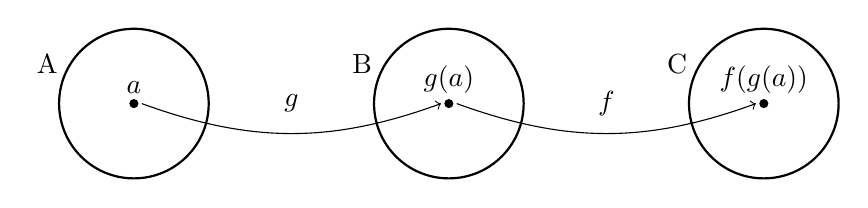
\begin{tikzpicture}
      \draw[thick] (1,0) circle [radius = 0.95] node at (-0.1, 0.5) {A};
      \draw[thick] (5,0) circle [radius = 0.95] node at (3.9, 0.5) {B};
      \draw[thick] (9,0) circle [radius = 0.95] node at (7.9, 0.5) {C};

      \draw[fill] (1,0) circle [radius = 0.05] node[above] {$a$};
      \draw[fill] (5,0) circle [radius = 0.05] node[above] {$g(a)$};
      \draw[fill] (9,0) circle [radius = 0.05] node[above] {$f(g(a))$};

      \draw[->] (1.1,0) to [out=340, in=200] (4.9,0) node at (3,0) {$g$};
      \draw[->] (5.1,0) to [out=340, in=200] (8.9,0) node at (7,0) {$f$};
\end{tikzpicture}
\end{center}
\bigskip

If $a\in A$ then $g(a)\in B$, which is the domain of $f$, so $g(a)$ can be plugged into $f$ to get $f(g(a))$, which is $\in C$. So, by applying $g$ and then $f$, we effectively create a single function from $A$ to $C$. This function is denoted as $f \circ g$ \footnote{This is read as "$f$ composed with $g$" or, more commonly "$f$ of $g$"; and not "fog".} and called the \emph{composition} of $f$ with $g$:

\bigskip
\begin{center}
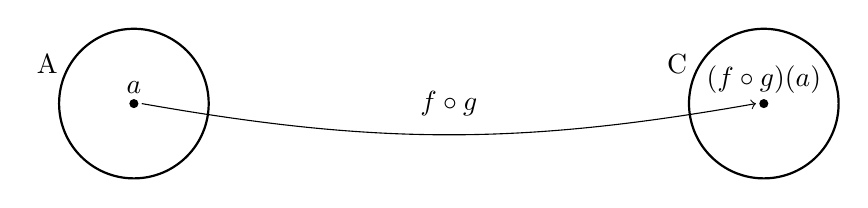
\begin{tikzpicture}
      \draw[thick] (1,0) circle [radius = 0.95] node at (-0.1, 0.5) {A};
      \draw[thick] (9,0) circle [radius = 0.95] node at (7.9, 0.5) {C};

      \draw[fill] (1,0) circle [radius = 0.05] node[above] {$a$};
      \draw[fill] (9,0) circle [radius = 0.05] node[above] {$(f\circ g)(a)$};

      \draw[->] (1.1,0) to [out=350, in=190] (8.9,0) node at (5,0) {$f\circ g$};
\end{tikzpicture}
\end{center}
\bigskip

\begin{dfn}
      Let $A, B,$ and $C$ be sets $g:A\rightarrow B$, and $f:B\rightarrow C$. Then the \emph{composition} function is denoted $f \circ g$ and is defined as thus:
      \[(f \circ g): A\rightarrow C \text{ where } (f \circ g)(a)=f(g(a)).  \]
      This composition function $f\circ g$ is a function from \underline{g's domain} to \underline{f's codomain}.
\end{dfn}




\bigskip \bigskip

\subsubsection{\underline{Proving injectiveness of $f\circ g$}}\hspace*{\fill}
\medskip


\begin{thrm}
      Suppose $A, B$ and $C$ are sets, $g:A\rightarrow B$ is injective, and $f:B\rightarrow C$ is injective. Then, $f\circ g$ is injective.
\end{thrm}

\noindent \textbf{Sketch Work.} We want to show that the function $f \circ g:A\rightarrow C$ is injective. Using the definition of injective, this means we want to show that given any $a_1,a_2\in A$, $(f\circ g)(a_1) = (f\circ g)(a_2)$ implies $a_1=a_2$. In other words, if $f(g(a_1))=f(g(a_2))$ then $a_1=a_2$. To prove this, therefore, we would have to begin from the outside function towards in and show that $f$ is injective first, then that $g$ is injective. Then we use the definition of a composition to prove that $f\circ g$ is injective.


Since the theorem says $f:B\rightarrow C$ is injective, we use the definition of injectiveness whereby for any $b_1,b_2\in B$, if $f(b_1)=f(b_2)$ then $b_1=b_2$. Since any two elements in $B$ wold satisfy this, and $g(a_1)$ and $g(a_2)$ are also elements of $B$, $f(g(a_1))=f(g(a_2))$ implies $g(a_1)=g(a_2)$.


Similarly the theorem states that $g:A\rightarrow B$ is injective. This means for any $a_1, a_2\in A$, if $g(a_1)=g(a_2)$ then $a_1=a_2$.

\begin{proof}
      Since $(f\circ g):A\rightarrow C$, to show that $f\circ g$ is injective, we must show that for any $a_1,a_2\in A$, if $(f\circ g)(a_1)=(f\circ g)(a_2)$ then $a_1=a_2$.


      Accordingly, assume $a_1,a_2\in A$ and $(f\circ g)(a_1)=(f\circ g)(a_2)$. If we apply the definition of composition function then we get
      \[f(g(a_1)) = f(g(a_2)).\]
      Since $f:B\rightarrow C$ is an injection, if $f(b_1)=f(b_2)$ for any $b_1,b_2\in B$ then $b_1=b_2$. In particular, observe that $g(a_1),g(a_2)\in B$ and $f(g(a_1))=f(g(a_2))$, and so $g(a_1)=g(a_2)$.


      Likewise, since $g:A\rightarrow B$ is injective, and we just showed that $g(a_1)=g(a_2)$ where $a_1,a_2\in A$. This implies that $a_1=a_2$.


      We have shown that for $a_1,a_2\in A$, if $(f\circ g)(a_1)=(f\circ g)(a_2)$, then $a_1=a_2$. Thus, $(f\circ g)$ is an injection.
\end{proof}





\bigskip \bigskip

\subsubsection{\underline{Proving surjectiveness of $f\circ g$}}\hspace*{\fill}
\medskip


\begin{thrm}
      Suppose $A, B$ and $C$ are sets, $g:A\rightarrow B$ is surjective, and $f:B\rightarrow C$ is surjective. Then, $f\circ g$ is surjective.
\end{thrm}

\noindent \textbf{Sketch Work.} Just like what we did in the last proof, we begin with the outer function and go inwards. In this case, surjectiveness means that for any $c\in C$ there exists some $a\in A$ such that $(f\circ g)(a)=c$.

\begin{proof}
      Assume $c \in C$. Since $f:B\rightarrow C$ is surjective and $c\in C$, there must be some $b\in B$ such that $f(b)=c$. Next, since $b\in B$ and $g:A\rightarrow B$ is surjective, there must be some $a\in A$ such that $g(a)=b$.
      Accordingly, for an arbitrary $c\in C$ we have found an $a\in A$ such that
      \[(f\circ g)(a) = f(g(a)) = f(b) = c, \]
      completing the proof.
\end{proof}
\bigskip
\emph{Corollary} is a result that follows quickly from previous results. The previous two theorems give the following corollary:
\bigskip
\noindent \textbf{Corollary.} Suppose $A,B$ and $C$ are sets, $g:A\rightarrow B$ is bijective, and $f:B\rightarrow C$ is bijective. Then $f\circ g$ is bijective.










\bigskip \bigskip \bigskip

\subsection{\underline{Invertibility}}\hspace*{\fill}
\bigskip

Similar to \emph{multiplicative identity} of 1 in the reals where $a\cdot 1=a$ for all $a\in\mathbb{R}$, and to \emph{additive identity} of 0, where $a+0=a$ for all $a\in\mathbb{R}$, there is also an \emph{identity function} which is analogous to 1 and 0 in the reals in that when you apply to any function, the function is unchanged. The difference is that the operation is a function composition instead of addition or multiplication. In this way, many functions will also have inverses.

\begin{dfn}
      For a set $A$, the \emph{identity function} on $A$ is the function
      \[i_A:A\rightarrow A \text{ where } i_A(x)=x \text{ for every } x\in A.\]
      The inverse of a function $f:A\rightarrow B$, if it exists, is the function $f^{-1}:B\rightarrow A$ such that $f^{-1}\circ f=i_A$ and $f\circ f^{-1}=i_B$.
\end{dfn}


For example, if $f:\mathbb{R}\rightarrow\mathbb{R}$ where $f(x)=x+1$, then $f^{-1}:\mathbb{R}\rightarrow\mathbb{R}$ is the function $f^{-1}(x)=x-1$. To see this, note that
\[(f\circ f^{-1})(x) = f(f^{-1}(x)) = f(x-1)+1 = x, \]
showing that $(f\circ f^{-1})(x)=x$, meaning that it is equal to the identity function $(i_\mathbb{R}(x)=x)$ on $\mathbb{R}$. Likewise,
\[(f^{-1}\circ f)(x) = f^{-1}(f(x)) = f^{-1}(x+1) = (x+1)-1 = x. \]

\bigskip
Here is another example:
\medskip
If $f:[0,1]\rightarrow [0,2]$ where $f(x)=2x$, then $f^{-1}:[0,2]\rightarrow [0,1]$ is the function $f^{-1}(x)=\frac{1}{2}x$.


Note that for a function to have an inverse, it \emph{must} be a bijection. That is, it must be an injection, \emph{and} a surjection. Recall in the definitions section above we defined when a function is not an injection and when a function is not a surjection. The diagrams are reproduced below for convenience:

\begin{center}
\begin{tabular}{l c}
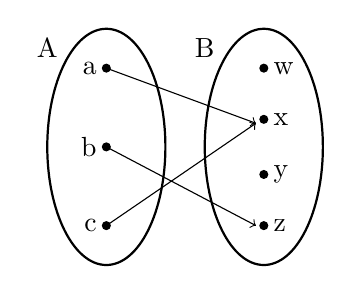
\begin{tikzpicture}
            \draw[thick] (2,0) ellipse (0.75cm and 1.5cm) node at (1.25, 1.25){A};
            \draw[thick] (4,0) ellipse (0.75cm and 1.5cm) node at (3.25, 1.25){B};

            \draw[fill] (2, 1) circle [radius=0.05] node[left]{a};
            \draw[fill] (2, 0) circle [radius=0.05] node[left]{b};
            \draw[fill] (2, -1) circle [radius=0.05] node[left]{c};

            \draw[fill] (4, 1) circle [radius=0.05] node[right]{w};
            \draw[fill] (4, 0.35) circle [radius=0.05] node[right]{x};
            \draw[fill] (4, -0.35) circle [radius=0.05]node[right]{y};
            \draw[fill] (4, -1) circle [radius=0.05] node[right]{z};

            \draw[->] (2,1) to (3.9, 0.3);
            \draw[->] (2,0) to (3.9,-1);
            \draw[->] (2,-1) to (3.9, 0.3);
      \end{tikzpicture}
      &
      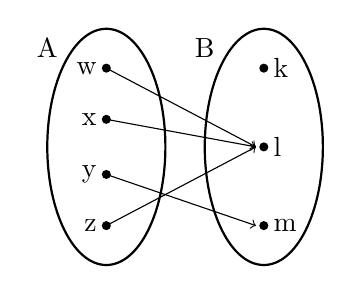
\begin{tikzpicture}
            \draw[thick] (6,0) ellipse (0.75cm and 1.5cm) node at (5.25, 1.25){A};
            \draw[thick] (8,0) ellipse (0.75cm and 1.5cm) node at (7.25, 1.25){B};

            \draw[fill] (6, 1) circle [radius=0.05] node[left]{w};
            \draw[fill] (6, 0.35) circle [radius=0.05] node[left]{x};
            \draw[fill] (6, -0.35) circle [radius=0.05] node[left]{y};
            \draw[fill] (6, -1) circle [radius=0.05] node[left]{z};

            \draw[fill] (8, 1) circle [radius=0.05] node[right]{k};
            \draw[fill] (8, 0) circle [radius=0.05] node[right]{l};
            \draw[fill] (8, -1) circle [radius=0.05] node[right]{m};

            \draw[->] (6,1) to (7.9, 0);
            \draw[->] (6,0.35) to (7.9,0);
            \draw[->] (6, -0.35) to (7.9, -1);
            \draw[->] (6, -1) to (7.9, 0);
      \end{tikzpicture} \\
    Not an injection from $A$ to $B$
    &
    Not a surjection from $A$ to $B$
\end{tabular}
\end{center}

\bigskip
In the left diagram above, $f^{-1}$ cannot send $x\in B$ to both $a$ and $c$ since a function has to send everything to only one destination. This is why $f$ must be injective in order for $f^{-1}$ to exist.


Similarly, in the right diagram above, $f^{-1}$ can't send $k\in B$ anywhere but a function has to send everything somewhere. This is why $f$ must be surjective in otder for $f^{-1}$ to exist.


The converse is also true. That is, every bijection is invertible.

\begin{thrm}
      A function $f:A\rightarrow B$ is invertible if and only if $f$ is a bijection.
\end{thrm}

\begin{proof}
      First suppose that $f:A\rightarrow B$ is invertible. We will prove that $f$ is both an injection and a surjection, which will prove that $f$ is therefore a bijection.


      To see that $f$ is a surjection, choose any $b\in B$. We aim to find an $a\in A$ such that $f(a)=b$. To this end, let $a=f^{-1}(b)$, which exists and is in $A$ because $f^{-1}:B\rightarrow A$. Observe that the definition of an invertible function implies
      \[f(a) = f(f^{-1}(b)) = b. \]
      This proves that $f$ is surjection.


      To see that $f$ is an injection, let $a_1,a_2\in A$ and assume $f(a_1)=f(a_2)$. Note that $f(a_1)$, as well as $f(a_2)$ by virtue of being equal to $f(a_1)$, is an element of B due to the fact that $f:A\rightarrow B$. And so, since $f^{-1}:B\rightarrow A$, we may apply $f^{-1}$ to both sides:
      \begin{align*}
            f(a_1)&=f(a_2) \\
            f^{-1}(f(a_1))&=f^{-1}(f(a_2)) \\
            a_1&=a_2,
      \end{align*}
      by the definition of inverse. Thus, $f$ is an injection. Since it is also surjection, it must be a bijection. This concludes the forward direction of the theorem.

      \bigskip
      As for the backwards direction, assume that $f$ is a bijection. For $b\in B$, we will now define $f^{-1}(b)$ as the following:
      \[f^{-1}(b)=a \text{ if } f(a)=b.\]
      That is we are defining $f^{-1}$ to act as we would want an inverse from $B$ to $A$ to act without yet claiming that $f^{-1}$ is a function.


      Our goal now is to demonstrate that this definition of $f^{-1}$ satisfies the conditions to be a function, which would prove that $f$ is invertible. To do so, recall that to be a function there is an existence condition whereby $f^{-1}(b)$ must be equal to some $a\in A$, and a uniqueness condition whereby $f^{-1}(b)$ must be equal to only one $a\in A$. We will check these separately:
      \medskip
      \underline{Existence:} Let $b\in B$. Since $f$ is surjective, there must be some $a\in A$ such that $f(a)=b$. Hence, by our definition of $f^{-1}$, we have $f^{-1}(b)=a$. We have shown that for every $b\in B$ there exists at least one $a\in A$ for which $f^{-1}(b)=a$, which concludes the existence portion of this argument.
      \smallskip
      \underline{Uniqueness:} Suppose $f^{-1}(b)=a_1$ and $f^{-1}(b)=a_2$, for some $b\in B$ and $a_1,a_2\in A$. By the definition of $f^{-1}$, this means that $f(a_1)=b$ and $f(a_2)=b$. However, since $f$ is injective, this means that $a_1=a_2$. We have shown that $f^{-1}(b)$ cannot be equal to two different elements of $A$, which concludes the uniqueness portion of this argument.


      Combined, these two parts show that $f^{-1}:B\rightarrow A$ is a function. Moreover, by the way we defined $f^{-1}$, we see that $f^{-1}(f(a))=a$ for all $a\in A$, and $f(f^{-1}(b))=b$ for all $b\in B$. Thus, by the definition of the inverse, $f^{-1}$ is the inverse function of $f$, proving that $f$ is invertible.


      We have proved the forwards and backwards directions of the Theorem which completes the proof.
\end{proof}


\end{document}
